\documentclass[tikz,border=10pt]{standalone}
\begin{document}
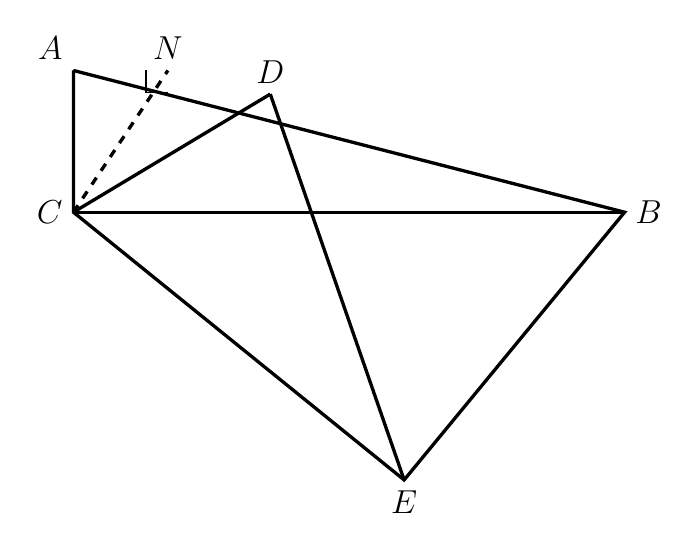
\begin{tikzpicture}[line width=1.2pt]
\coordinate (A) at (0,4);
\coordinate (N) at (1.2,4);
\coordinate (D) at (2.5,3.7);
\coordinate (C) at (0,2.2);
\coordinate (B) at (7,2.2);
\coordinate (E) at (4.2,-1.2);

\draw (A) -- (C) -- (E) -- (B) -- (A);
\draw (C) -- (B);
\draw (C) -- (D);
\draw (D) -- (E);

\draw[dashed] (C) -- (N);

% right angle mark at N
\draw[line width=0.6pt] (N) ++(-0.28,0) -- ++(0,-0.28) -- ++(0.28,0);

\foreach \L/\pos in {A/{above left},N/{above},D/{above},C/{left},B/{right},E/{below}} {
  \node[\pos, font=\large] at (\L) {$\L$};
}
\end{tikzpicture}
\end{document}
